\section{Numerical Framework for Rubber-like Materials} \label{general}
In this section, we briefly review the decomposition of hyperelastic models, the general method to derive stress and elasticity tensor, the principle of virtual work, principle of stationary energy and its linearization. Thses topics cover the complete process of deriving the displacement-based formulation and mixed formulation for hyperelastic material. Inserting a specific hyperelastic model, following the steps in this section, as shown in Figure \ref{fig:flowchart}, we will derive an incremented linear system to solve for our unknowns. 
\begin{figure}[h!]
\centering
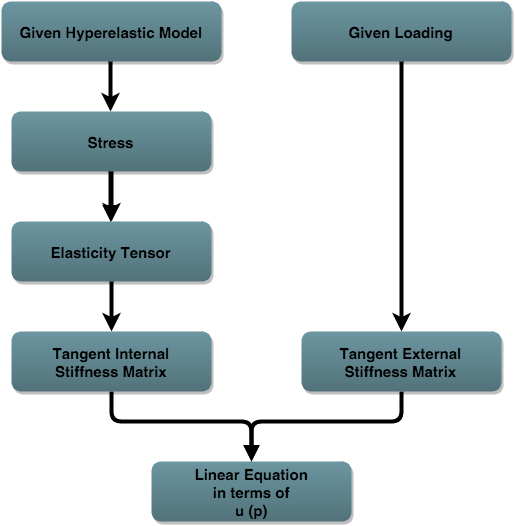
\includegraphics[width=.6\textwidth]{./figures/flowchart.png}
\caption{Procedures to Follow}
\label{fig:flowchart}
\end{figure}

%
\subsection{Hyperelastic Model}
Generally in continuum mechanics we use constitutive equations to describe the stress components in terms of other functions such as strain. This functional relationship distinguishes different types of materials. One important type of materials that is widely used in biomechanics is hyperelastic material. For hyperelastic material, we postulate there exists a Helmholtz free-energy function $\Psi$, which is defined per unit reference volume. If $\Psi$ is uniquely determined by deformation tensor $\bold{F}$ or other strain tensor, it is called strain-energy function. If the strain is given, the stress can be uniquely determined from the strain-energy function.  

Our discussion will be focused on rubber-like materials which are modeled as incompressible or nearly incompressible. The tensors related to the deformation are usually split into a volumetric part and an isochoric part. The motivation is to let the determinant of the isochoric part to be $1$ so that it represents a volume-keeping component. For example, the deformation tensor $F$ and the right Cauchy-Green tensor $\bold{C}$ are decomposed as
\begin{equation} \label{split1}
\bold{F} = (J^{1/3}\bold{I})\overline{\bold{F}}
\qquad
\bold{C} = (J^{2/3}\bold{I})\overline{\bold{C}}
\end{equation}
where $J$ is the determinant of deformation tensor $\bold{F}$. The terms $J^{1/3}\bold{I}$ and $J^{2/3}\bold{I}$ are the volumetric parts while $\overline{\bold{F}}$ and $\overline{\bold{C}}$ are the isochoric parts. $\overline{\bold{F}}$ and $\overline{\bold{C}}$ are also referred as modified deformation tensor and modified right Cauchy-Green tensor. Meanwhile, the strain-energy function is postulated to have a unique decoupled form
\begin{equation} \label{split2}
\Psi(\bold{C}) = \Psi_{vol}(J) + \Psi_{iso}(\overline{\bold{C}})
\end{equation}
where $\Psi_{vol}(J)$ and $\Psi_{iso}(\overline{\bold{C}})$ are volumetric and isochoric response of the material respectively. For incompressible models, the volumetric part of the strain-energy function acts as a Lagrange condition to enforce the incompressibility $J -1 = 0$.
\begin{equation} \label{Lagrange}
\Psi_{vol} = p(J-1)
\end{equation} 
where $p$ is a Lagrange multiplier and can be identified as hydrostatic pressure. It cannot be uniquely determined from the deformation. Instead, it has to be determined from the equilibrium equation and boundary conditions. For compressible material, the volumetric part of the strain-energy function is a penalty to allow a small compressibility.
\begin{equation} \label{penalty}
\Psi_{vol} = \kappa{G(J)}
\end{equation}
where $\kappa$ is the penalty parameter and can be interpreted as the bulk modulus, $G(J)$ is the penalty function and may adopt the simple form
\begin{equation} \label{penalty2}
G(J) = \frac{1}{2}(J(\bold{u}) - 1 )^2
\end{equation}

%
\subsection{Stress Evaluation}
Based on the postulation of strain-energy function, it follows that the work done on hyperelastic materials in a dynamical process within a time interval $[t_1, t_2]$ is the difference between the strain-energy in two states. It can also be proved that the work can be written as the integration of the tensor product of conjugate stress-strain rate pairs.
\begin{equation}
\Psi({\bold{F_2}}) - \Psi({\bold{F_1}}) = \delta{W_{int}} = \int_{t_1}^{t_2}\bold{P}:\dot{\bold{F}}dt = \int_{t_1}^{t_2}\bold{S}:\dot{\bold{E}}dt = 
\int_{t_1}^{t_2}\boldsymbol{\sigma}:\dot{\bold{e}}dt
\end{equation}
where $\bold{P}$ is the first Piola-Kirchhoff stress, $\bold{S}$ is the second Piola-Kirchhoff (PK2) stress tensor, $\bold{E}$ is the Green-Lagrange strain tensor and $\bold{e}$ is Euler-Almansi strain tensor which is defined as the symmetric part of the gradient of displacement in current configuration, i.e., $\delta\bold{e} = \frac{1}{2}{ grad^T\delta\bold{u} + grad\delta\bold{u}}$.

If the material is homogeneous, the PK2 stress $\bold{S}$ can be determined by 
\begin{equation}
\bold{S} = 2\frac{\partial\Psi(\bold{C})}{\partial{\bold{C}}} = \frac{\partial\Psi(\bold{E})}{\partial{\bold{E}}}
\end{equation}
Furthermore, if the material is isotropic, the PK2 stress can be expressed as a function of the three invariants of right (or left) Cauchy-Green tensor
\begin{equation} \label{PK2}
\bold{S} = 2\frac{\partial\Psi({\bold{C})}}{\partial{\bold{C}}} = 2\left[\left( \frac{\partial\Psi}{\partial{I_1}} + I_1 \frac{\partial\Psi}{\partial{I_2}} \right)\bold{I} -  \frac{\partial\Psi}{\partial{I_2}}\bold{C} + I_3 \frac{\partial\Psi}{\partial{I_3}}{\bold{C}}^{-1} \right]
\end{equation}
where $I_1 = tr(\bold{C}) = tr(\bold{B})$, $I_2 = \frac{1}{2}(I_1^2 - tr(\bold{B}^2))$, and $I_3 = det(\bold{C}) = det(\bold{B}) = J^2$ are three invariants of the right Cauchy-Green tensor $\bold{C}$ or the left Cauchy-Green tensor $\bold{B}$. $I_1$ and $I_2$ also have their modified counterparts $\bar{I_1} = J^{-2/3}I_1$, $\bar{I_2} = J^{-4/3}I_2$. But there are also constitutive models written as function of principal stretches instead of invariants. For instance Odgen's model. In this case the invariants must be replaced by principal stretches in Equation \ref{PK2}.

Correspondingly, the PK2 stress can be split into a volumetric part and a isochoric part
\begin{equation} \label{S}
\bold{S} =  2\frac{\partial{\Psi({\bold{C})}}}{\partial{\bold{C}}} = \bold{S_{vol}}  + \bold{S_{iso}} 
\end{equation}
\begin{equation} \label{Svol}
\bold{S_{vol}} = 2\frac{\partial{\Psi(J)}}{\partial{\bold{C}}} = Jp{\bold{C}} ^{-1}
\end{equation}
\begin{equation} \label{Siso}
\begin{split}
\bold{S_{iso}} & = 2\frac{\partial{\Psi({\bold{C})}}}{\partial{\bold{C}}} = J^{-2/3}(\mathbb{I} - \frac{1}{3}\bold{C}^{-1} \otimes \bold{C}):\overline{\bold{S}} \\
&  = J^{-2/3}Dev\overline{\bold{S}} = J^{-2/3}\mathbb{P}:\overline{\bold{S}}
\end{split}
\end{equation}
where  $\overline{\bold{S}}$ is the fictitious PK2 stress defined by
\begin{equation} \label{fictitious}
\overline{\bold{S}} = 2\frac{\partial\Psi_{iso}({\overline{\bold{C}})}}{\partial\overline{\bold{C}}}
\end{equation}
and $\mathbb{P}$ is the projection tensor defined by $\mathbb{P} = \mathbb{I} - \frac{1}{3}\bold{C}^{-1} \otimes \bold{C} $. $\mathbb{I}$ is the fourth order identity tensor. The symbol $Dev$ is an operator defined as $Dev(\bullet) = \mathbb{P}:(\bullet)$.

Note that for incompressible material, the hydrostatic pressure $p$ is independent of the displacement and has to be determined from equilibrium equation and boundary conditions. However, for compressible material,  $p$ is a function of displacement although it can be treated as an independent variable, and can be determined by the constitutive law
\begin{equation} \label{pressure}
p = \frac{d\Psi_{vol}(J)}{dJ}
\end{equation}
If we leave $p$ as an unknown and implement Equation \ref{pressure} as additional constraint, we will have a displacement/pressure mixed formulation. If we replace $p$ with $\bold{u}$ using Equation \ref{pressure}, we end up with a displacement-base formulation.

%
\subsection{Elasticity Tensor}
The solutions in nonlinear finite element methods are often obtained incrementally with Newton's method. The elasticity tensors is crucial in the implementation of Newton's method.
In the material description (reference configuration), the elasticity tensor is defined as the gradient of the PK2 stress to its work conjugate strain, which is Green-Lagrange strain.
\begin{equation}
\mathbb{C} = \frac{\partial{\bold{S}(\bold{E})}}{\partial{\bold{E}}} =  2\frac{\partial{\bold{S}(\bold{C})}} {\partial{\bold{C}}} = 4 \frac{\partial^2{\Psi(\bold{C})}}{{\partial{\bold{C}}}{\partial{\bold{C}}}}
\end{equation}
Based on the split of deformation tensors in Equation \ref{split1} and the assumption in Equation \ref{split2}, the elasticity tensors can be rewritten in the decoupled form
\begin{equation} \label{C}
\mathbb{C} = 2\frac{\partial{\bold{S}}}{\partial{\bold{C}}} = \mathbb{C}_{vol} + \mathbb{C}_{iso} 
\end{equation}
\begin{equation} \label{Cvol}
\mathbb{C}_{vol} = 2\frac{\partial{\bold{S}_{vol}}}{\partial{\bold{C}}}
\quad
\mathbb{C}_{iso} = 2\frac{\partial{\bold{S}_{iso}}}{\partial{\bold{C}}}
\end{equation}
Substituting Equation \ref{Svol} and \ref{Siso}  into these, we can obtain the expressions for $\mathbb{C}_{vol}$ and $\mathbb{C}_{iso}$ .
\begin{equation} \label{Cvol}
\mathbb{C}_{vol} = J\tilde{p}\bold{C}^{-1}\otimes\bold{C}^{-1} - 2Jp\bold{C}^{-1}\odot\bold{C}^{-1}
\end{equation}
\begin{equation} \label{Ciso}
\mathbb{C}_{iso} = \mathbb{P} : \overline{\mathbb{C}} : \mathbb{P}^T + \frac{2}{3}Tr(J^{-2/3}\overline{\bold{S}})\tilde{\mathbb{P}} - \frac{2}{3}(\bold{C}^{-1}\otimes\bold{S}_{iso} + \bold{S}_{iso}\otimes \bold{C}^{-1})
\end{equation}
where $\otimes$ denotes the dyadic product, $\odot$ is defined as the derivative of the inverse of a second order tensor with respect to itself, i.e.
\begin{equation}\label{dyadic}
{(\bold{A} \otimes \bold{B})}_{ijkl} = {\bold{A}}_{ij}{\bold{B}}_{kl}
\end{equation}
\begin{equation} \label{circlecc}
\bold{C}^{-1}\odot\bold{C}^{-1} = - \frac{\partial{\bold{C}^{-1}}}{\partial{\bold{C}}}
\end{equation}
$\tilde{p}$, $\overline{\mathbb{C}}$, $\tilde{\mathbb{P}}$ and $Tr(\bullet)$ are defined as
\begin{equation} \label{tildep}
\tilde{p} = p + J\frac{dp}{dJ}
\end{equation}
\begin{equation} \label{barcc}
\overline{\mathbb{C}} = 2J^{-4/3}\frac{\partial^2\Psi_{iso}(\overline{\bold{C}})}{\partial{\overline{\bold{C}}}{\partial{\overline{\bold{C}}}}}
\end{equation}
\begin{equation} \label{tildepp}
\tilde{\mathbb{P}} = \bold{C}^{-1} \odot \bold{C}^{-1} -  \frac{1}{3}\bold{C}^{-1} \otimes \bold{C}^{-1} 
\end{equation}

\begin{equation} \label{tracec}
Tr(\bullet) = (\bullet) : \bold{C}
\end{equation}
Plug in a specific model of Equation \ref{split2} and its corresponding Equations $(\ref{S} - \ref{Siso})$ into Equations \ref{C}, \ref{Cvol} and \ref{Ciso}, we can obtain the elasticity tensor. Note that for incompressible material, $\tilde{p} = p$ because $p$ is independent of $J$.

%
\subsection{Principle of Virtual Work} \label{PVW}
The variational approach is the cornerstone for finite element methods. The most fundamental variational principle that origins from Newton's law is the principle of virtual work. Neglecting the kinematic term, it can be written as
\begin{equation} \label{basic}
\delta{W_{int}} = \delta{W_{ext}}
\end{equation}
\begin{equation} \label{Wint}
\delta W_{int}(\bold{u}, \delta\bold{u}) = \int_\Omega \boldsymbol\sigma : \delta\bold{e}dv = \int_{\Omega_{0}}\bold{S} : \delta\bold{E}dV
\end{equation}
\begin{equation} \label{Wext}
\delta W_{ext}(\bold{u}, \delta\bold{u}) = \int_\Omega\bold{b}\cdot\delta\bold{u}dv +  \int_{\partial\Omega}\overline{\bold{t}}\cdot\delta{\bold{u}}ds = \int_\Omega\bold{B}\cdot\delta\bold{u}dV +  \int_{\partial{\Omega_0}}\overline{\bold{T}}\cdot\delta{\bold{u}}dS
\end{equation}
The internal work is done by Cauchy stress $\bold\sigma$ along the virtual Euler-Almansi strain $\delta\bold{e}$ about region $\Omega$ and the external work is done by the body force $\bold{b}$ and the surface traction $\overline{\bold{t}}$, along the virtual displacement $\delta{u}$ about region $\Omega$ and its boundary surface $\partial\Omega$ respectively. They are assumed be mapped to the reference configuration. 

If the external loading is given as fixed traction in reference configuration, the virtual external work is constant. Example for this type of loading is tension test where the external force with respect to reference configuration is given as a constant. Another type of loading, which is more frequently encountered in biomechanics is the fixed pressure loading.
In this case, the pressure on the current boundary surface is constant, i.e. $\overline{\bold{t}} = \boldsymbol{\sigma{n}} = p\bold{n}$ where p is a given constant, $\bold{n}$ is the unit normal vector of the current surface. The external virtual work done by the constant pressure $p$ along the virtual displacement $\delta{\bold{u}}$ is defined by
\begin{equation} \label{Wext2}
\delta{W_{ext}}(\bold{u}, \delta{\bold{u}}) = p\int_{\partial\Omega} \bold{n}\cdot\delta{\bold{u}}ds
\end{equation}

%
\subsection{Principle of Stationary Potential Energy}
Assuming the mechanical system is conservative, there exists an energy functional $\Pi$ for both the stresses and the loadings. Their sum is constant. In the displacement-based formulation, $\Pi$ is a function of $\bold{u}$ only, and it leads to the same equations as the virtual work balance. While in the displacement/pressure mixed formulation, $\Pi$ is a function of both $\bold{u}$ and $p$. It treats pressure as an independent variable and has advantages of avoiding locking and ameliorate the ill-condition of the stiffness matrix in certain situation.

In displacement-based formulation, the potential energy is expressed as
\begin{equation}
\Pi(\bold{u}) = \Pi_{int}(\bold{u}) + \Pi_{ext}(\bold{u})
\end{equation}
\begin{equation} \label{pint}
\Pi_{int}(\bold{u}) = \int_{\Omega_{0}}\Psi(\bold{F}(\bold{u}))dV
\end{equation}
\begin{equation} \label{pext}
\Pi_{ext}(\bold{u}) =  - \int_\Omega\bold{B}\cdot\bold{u}dV -  \int_{\partial{\Omega_0}}\overline{\bold{T}}\cdot{\bold{u}}dS
\end{equation}
Our objective is to find the state of equilibrium for which the system is stationary. In displacement-based formulation, this means the directional derivative with respect to the displacement $\bold{u}$ to vanish in all directions $\delta{\bold{u}}$.
\begin{equation} \label{equilibrium}
D_{\delta\bold{u}}\Pi(\bold{u}) = D_{\delta\bold{u}}\Pi_{int}(\bold{u}) + D_{\delta\bold{u}}\Pi_{ext}(\bold{u}) = 0
\end{equation} 
 In other words, we require the first variation of the total energy potential $\delta\Pi$ to vanish.
 \begin{equation} \label{potential}
\delta\Pi(\bold{u}, \delta\bold{u}) =\delta\Pi_{int}(\bold{u}) + \delta\Pi_{ext}(\bold{u}) = 0
\end{equation}
Here we adopt the convention in Holzapfel using $D_{\Delta{x}}f(x, y, \textit{etc.})$ to represent the directional derivative of $f$ as a function of $(x, y, \textit{etc.})$ along the direction of $\Delta{x}$ where $x$, $y$, \textit{etc.} can be scalar or tensor of any other order. The directional derivative $D_{\Delta{x}}f(x, y, \textit{etc.})$ is equivalent to the first variation of functional $f$ with respect to $x$.
Equation \ref{equilibrium} or \ref{potential} is the equation we want to solve in the displacement-based formulation. It is easy to prove the following equivalence
\begin{equation}
D_{\delta\bold{u}}\Pi_{int}(\bold{u}) = \delta W_{int}(\bold{u}, \delta\bold{u}) \quad
D_{\delta\bold{u}}\Pi_{ext}(\bold{u}) = - \delta W_{ext}(\bold{u}, \delta\bold{u})
\end{equation}
So that Equation \ref{equilibrium} or \ref{potential} is equivalent to Equation \ref{basic}. 

In mixed formulation, we have two independent variables, $\bold{u}$ and $p$. The state of equilibrium is with respect to both of them. Our objective equation becomes
\begin{equation} \label{target}
D_{\delta\bold{u}}\Pi(\bold{u}, p) = 0 \quad D_{\delta{p}}\Pi(\bold{u}, p) = 0
\end{equation}
To summarize, in displacement-based formulation, our goal is to find an equilibrium state for total potential energy with respect to $\bold{u}$; in mixed formulation, we need to find an equilibrium state with respect to both $\bold{u}$ and $p$. To solve these equations, we have to linearize them first. That is, finding the second variation of potential energy.


%
\subsection{Linearization of Principle of Stationary Potential Energy}
In displacement-based formulation, we want to solve Equation \ref{equilibrium}. Based on Equation \ref{Wint}, by means of differentiation, we have
\begin{equation} \label{Kint}
D_{\delta\bold{u}, \Delta\bold{u}}\Pi_{int}^2(\bold{u}) = D_{\Delta{\bold{u}}}\delta{W_{int}}(\bold{u}, \delta{\bold{u}}) = \int_{\Omega_0}(Grad\delta\bold{u} : Grad\Delta\bold{u}\bold{S} + \bold{F}^TGrad\delta{u} : \mathbb{C} : \bold{F}^T Grad\Delta\bold{u})dV
\end{equation}
The first part of the integration is called initial stress contribution since the $\bold{S}$ characterize the initial stress at every increment. The second part is called material contribution because the $\mathbb{C}$ characterize the material response to the displacement.

As discussed in Section \ref{PVW}, for the first type of external loading as in  Equation \ref{Wext}, the external work is independent of the displacement. So the variation vanishes.
\begin{equation} \label{Kext}
D_{\delta\bold{u}, \Delta\bold{u}}\Pi_{ext}^2(\bold{u}) = - D_{\Delta{\bold{u}}}\delta{W_{ext}}(\bold{u}, \delta{\bold{u}}) = 0
\end{equation}
But for the second type of loading as in Equation \ref{Wext2}, the external work is changing with the current configuration due to the change of normal $\bold{n}$ and integration area $ds$. 

Let $\bold{x}$ be an arbitrary point on the surface of a 3D element, $\xi$ and $\eta$ be the parent coordinates on that surface. Then the unit normal vector of that surface $\bold{n}$ as well as the infinite small area $ds$ can be expressed as
\begin{equation}
\bold{n} = \frac{  \frac{\partial{\bold{x}}}{\partial{\xi}} \times  \frac{\partial{\bold{x}}}{\partial{\eta}} }{\left| \frac{\partial{\bold{x}}}{\partial{\xi}} \times  \frac{\partial{\bold{x}}}{\partial{\eta}} \right|}
\end{equation}
\begin{equation}
ds = \left|\frac{\partial{\bold{x}}}{\partial{\xi}} \times  \frac{\partial{\bold{x}}}{\partial{\eta}}\right| d\xi{d\eta}
\end{equation}
With these two equations, we can express Equation \ref{Wext2} as
\begin{equation}
\delta{W_{ext}}(\bold{u}, \delta{\bold{u}}) = p\int_{\Omega_{\xi}}  \left(\frac{\partial{\bold{x}}}{\partial{\xi}} \times  \frac{\partial{\bold{x}}}{\partial{\eta}}\right) \cdot\delta{\bold{u}}d\xi{d\eta}
\end{equation}
The linearization is obtained by a straight-forward derivation with respect to $\Delta\bold{u}$. 
\begin{equation}  \label{Kext2}
D_{\delta\bold{u}, \Delta\bold{u}}\Pi_{ext}^2(\bold{u}) = - D_{\Delta{\bold{u}}}\delta{W_{ext}}(\bold{u}, \delta{\bold{u}}) = - p\int_{\Omega_{\xi}}  \left(\frac{\partial{\bold{x}}}{\partial{\eta}} \times \delta\bold{u}\right) \cdot\Delta{\bold{u}}_{,\xi} - 
\left(\frac{\partial{\bold{x}}}{\partial{\xi}} \times \delta\bold{u}\right) \cdot\Delta{\bold{u}}_{,\eta} d\xi{d\eta}
\end{equation}
With Equation \ref{Kint} and \ref{Kext} or \ref{Kext2} we are able to obtain the matrix form for displacement-based formulation.
\begin{equation} \label{matrix}
\left( D_{\delta\bold{u}, \Delta\bold{u}}\Pi_{int}^2(\bold{u}) + D_{\delta\bold{u}, \Delta\bold{u}}\Pi_{ext}^2(\bold{u})  \right) \Delta\bold{u} = D_{\delta\bold{u}}\Pi_{int}(\bold{u}) + D_{\delta\bold{u}}\Pi_{ext}(\bold{u})
\end{equation}
The terms in the parenthesis on the lefthand side is the tangent stiffness matrix, the righthand side is the residual of the system potential energy. $\Delta\bold{u}$ is the increment of displacement. 

To solve Equation \ref{target}, linearization with respect to $\bold{u}$ and $p$ must be carried out. The incremented matrix form becomes
\begin{equation} \label{linear}
\begin{bmatrix}
D_{\delta\bold{u}, \Delta\bold{u}}^2 \Pi(\bold{u}, p)  && D_{\delta\bold{u}, \Delta{p}}^2 \Pi(\bold{u}, p)  \\ D_{\delta{p}, \Delta\bold{u}}^2 \Pi(\bold{u}, p)  && D_{\delta{p}, \Delta{p}}^2 \Pi(\bold{u}, p) 
\end{bmatrix}
\begin{bmatrix}
\Delta\bold{u} \\ \Delta{p}
\end{bmatrix}
= 
\begin{bmatrix}
D_{\delta\bold{u}}\Pi(\bold{u}, p) \\ D_{\delta{p}}\Pi(\bold{u}, p) 
\end{bmatrix}
\end{equation}
We inspect the righthand side first. For incompressible material, recall Equation \ref{split2} and \ref{Lagrange}, the energy potential is expressed as
\begin{equation} \label{split3}
\Pi_{int}(\bold{u}, p) = \int_{\Omega_0} \left[ p(J(\bold{u}) - 1) + \Psi_{iso}(\overline{\bold{C}}(\bold{u}))\right] dV
\end{equation}
Using the chain rule, it can be derived that
\begin{equation}\label{rhs1}
D_{\delta\bold{u}}\Pi(\bold{u}, p) = \int_{\Omega_0}\left( J(\bold{u})p\bold{C}^{-1}(\bold{u}) + 
2\frac{\partial{\Psi_{iso}(\overline{\bold{C}}(\bold{u}))}}{\partial{\bold{C}}}  \right) : \delta\bold{E}(\bold{u}) dV + D_{\delta\bold{u}}\Pi_{ext}(\bold{u})
\end{equation}
\begin{equation}\label{rhs2}
D_{\delta{p}}\Pi(\bold{u}, p) = \int_{\Omega_0} (J(\bold{u}) - 1 )\delta{p} dV
\end{equation}
For the left hand side, $D_{\delta\bold{u}, \Delta\bold{u}}^2 \Pi(\bold{u}, p)$ has already been derived in the last section as the sum of Equation \ref{Kint} and Equation \ref{Kext} or \ref{Kext2}, i.e.
\begin{equation} \label{lhs0}
D_{\delta\bold{u}, \Delta\bold{u}}^2 \Pi(\bold{u}, p) =  \int_{\Omega_0}(Grad\delta\bold{u} : Grad\Delta\bold{u}\bold{S} + \bold{F}^TGrad\delta{u} : \mathbb{C} : \bold{F}^T Grad\Delta\bold{u})dV  \end{equation}
when pressure boundary condition is applied
\begin{equation} \label{lhs1}
\begin{split}
D_{\delta\bold{u}, \Delta\bold{u}}^2 \Pi(\bold{u}, p) = & \int_{\Omega_0}(Grad\delta\bold{u} : Grad\Delta\bold{u}\bold{S} + \bold{F}^TGrad\delta{u} : \mathbb{C} : \bold{F}^T Grad\Delta\bold{u})dV  \\
 - & p\int_{\Omega_{\xi}}  \left(\frac{\partial{\bold{x}}}{\partial{\eta}} \times \delta\bold{u}\right) \cdot\Delta{\bold{u}}_{,\xi} - 
\left(\frac{\partial{\bold{x}}}{\partial{\xi}} \times \delta\bold{u}\right) \cdot\Delta{\bold{u}}_{,\eta} d\xi{d\eta}
\end{split}
\end{equation}
It is a little tricky but not complicated to obtain that
\begin{equation} \label{lhs2}
D_{\delta\bold{u}, \Delta{p}}^2 \Pi(\bold{u}, p) = \int_{\Omega_0} J(\bold{u})\Delta{p}div\delta{\bold{u}}dV
\end{equation}
\begin{equation} \label{lhs3}
D_{\delta{p}, \Delta\bold{u}}^2 \Pi(\bold{u}, p) = \int_{\Omega_0} J(\bold{u})div\Delta{\bold{u}}\delta{p}dV
\end{equation}
Since $\Pi$ is a first order function with respect to $p$, we have
\begin{equation} \label{lhs4}
D_{\delta{p}, \Delta{p}}^2 \Pi(\bold{u}, p) = 0
\end{equation}
Inserting Equation \ref{rhs1} to \ref{lhs4} into Equation \ref{linear} we can obtain a symmetric tangent stiffness matrix. Since $p$ is arbitrary for incompressible material, we need additional reference values for it to solve \ref{equilibrium}.

While for nearly incompressible material, Equation \ref{lhs4} and \ref{rhs2} need to be modified. Recall Equation \ref{penalty} and \ref{pressure}, the incompressibility condition is no longer strictly enforced. Equation \ref{rhs2} is relaxed to
\begin{equation} \label{relation}
D_{\delta{p}}\Pi(\bold{u}, p) = \int_{\Omega_0}\left(  \frac{dG(J(\bold{u}))}{dJ} - \frac{p}{\kappa} \right)\delta{p}dV = 0
\end{equation}
which reflects that $p$ is not arbitrary but related to $\bold{u}$.  
Accordingly, the second variation on $p$ is no longer $0$. Equation \ref{lhs4} is modified as
\begin{equation} \label{lhs42}
D_{\delta{p}, \Delta{p}}^2 \Pi(\bold{u}, p) = - \int_{\Omega_0}\frac{1}{\kappa}\Delta{p}\delta{p}dV
\end{equation}
Equation \ref{lhs1} to \ref{lhs3} and Equation \ref{rhs1} remain the same. The linear equation is closed, we do not need additional information on $p$.

















